\documentclass[a4paper]{instrumentacao}

\usepackage{listings}
\usepackage{etoolbox}
\usepackage{graphicx}

\newtoggle{attachments}
\togglefalse{attachments}

\graphicspath{
	{../Resources/Images/}
	{../Resources/Mathematica/images/}
	{../Resources/MATLAB/images/}
}

%todo colocar um titulo "criativo"
\title{Termometria}
\author{Rogiel Sulzbach \and Rodrigo de Castro Silveira \and Yi Chen Wu}
\startdate{}
\finishdate{}
\emails{
	\emailaddress{R.J.S.}{rogiel@rogiel.com},
	\emailaddress{R.C.S.}{csilveira.rodrigo@gmail.com} e
	\emailaddress{Y.C.}{yichenpoa@gmail.com}
}
\resume{}
\abstract{}
\keywords{}
\institute{Universidade Federal do Rio Grande do Sul, Departamento de Engenharia Elétrica, Curso de Engenharia Elétrica, Instrumentação A, Profs. Dr. Alexandre Balbinot e Dra. Léia Bagesteiro}

\headertext{Efeitos físicos}

\begin{document}
\maketitle


\chapter{Introdução}
% ...

\chapter{Metodologia Experimental}

\section{Calibração do sensor Pt100}
Pt100 é o nome dado à um tipo de termoresistor composto de Platina cuja resistência à temperatura de 0ºC é $100 \Omega$ a relação entre a resistência elétrica e a temperatura do componente é associada de forma direta e linear. Este último que torna a criação de um termômetro eletrônico algo trivial que possa ser implementado de forma simples e direta.

De acordo com \todo{referencia}, a função de transferência teórica do Pt100 é dada pela Equação \ref{eq:pt100}:

\begin{equation}
	R(T) \approxeq R_0 \left[1 + \alpha\left(T - T_0\right)\right]
	\label{eq:pt100}
\end{equation}

\noindent
onde $R(T)$ é a resistência elétrica do Pt100 para uma dada temperatura $T$, $\alpha$ é uma constante dependente de características de construção do Pt100, $R_0$ é a resistência de referência (tipicamente $100 \Omega$ para o Pt100) e $T_0$ é a temperatura de referência do termoresistor (tipicamente $0ºC$ para o Pt100).

Para estimar a função de transferência experimental do termoresistor, projetou-se um experimento onde foram feitas 2 medidas de forma aleatória para temperaturas de $18ºC$ até $78ºC$ graduadas em $2ºC$ cada. Na Figura \ref{fig:pt100-esquematico} está apresentado um desenho simplificado da configuração utilizada no experimento.

\begin{figure}[H]
\center
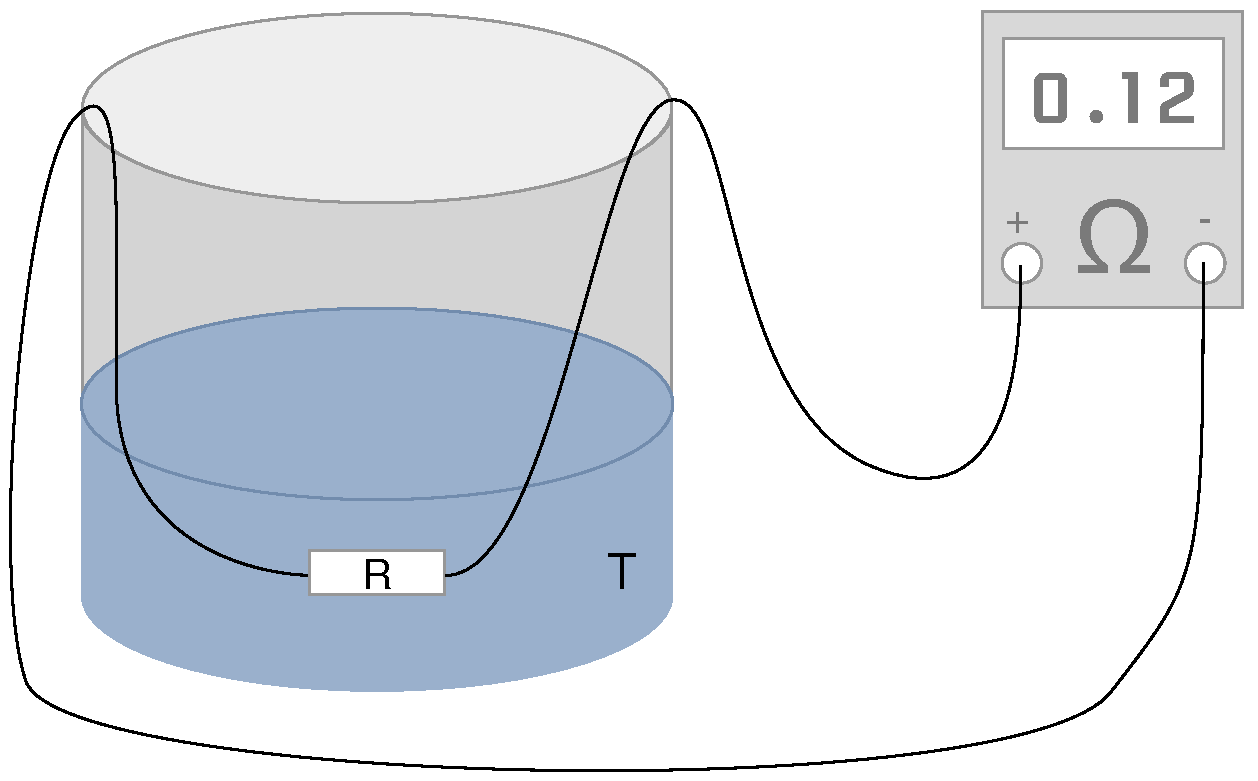
\includegraphics[width=\textwidth]{Bequer.pdf}
\caption{Desenho esquemático do experimento -- dentro de um béquer é colocada água com temperatura variando de $18ºC$ à $78ºC$ e mede-se a resistência elétrica correspondente do termoresistor.}
\label{fig:pt100-esquematico}
\end{figure}

\noindent
onde $R$ é um resistor Pt100, $T$ é a temperatura da água dentro do copo de Béquer, e o instrumento $\Omega$ é um ohmímetro.

\chapter{Resultados e Discussões}

\chapter{Conclusões}


\newpage
\begin{thebibliography}{9}
\bibitem{mathematica-numerial-precision} \url{https://reference.wolfram.com/language/tutorial/NumericalPrecision.html}, acessado em 16 de março de 2016

\bibitem{datasheet-lm7905} Datasheet oferecido pelo fabricante do regulador de tensão LM7905PI, disponível em \url{http://www.datasheetlib.com/datasheet/190159/kia7905pi_kec-korea-electronics-corporation.html}.

\bibitem{datasheet-lm7805} Datasheet oferecido pelo fabricante do regulador de tensão LM7805CV, disponível em \url{http://www.datasheetlib.com/datasheet/221840/l7805cv_stmicroelectronics.html}.

\bibitem{datasheet-lm741} Datasheet oferecido pelo fabricante do amplificador operacional LM741, disponível em \url{http://www.datasheetlib.com/datasheet/818655/lm741_ti-texas-instruments.html}.


%\bibitem{ref1} Sobrenome, A.B.; Sobrenome, C.D. Title of the cited article. Journal Title 2007, 6, 100-110. 
%\bibitem{ref2} Balbinot, A.; Brusamarello, V.J.. Title of the cited article. Journal Title 2007, 6, 100-110. 
%\bibitem{ref3} Author, A.; Author, B. Title of the chapter. In Book Title, 2nd ed.; Editor, A., Editor, B., Eds.; Publisher: Publisher Location, Country, 2007; Volume 3, pp. 154-196.
%\bibitem{ref4} Author, A.; Author, B. Book Title, 3rd ed.; Publisher: Publisher Location, Country, 2008; 
%pp. 154-196.

\end{thebibliography}

\iftoggle{attachments}{
	\chapter*{Anexos}
	\section{Mathematica}
	\includenotebook{../Resources/Mathematica/Experimento 1-1.nb.pdf}{Pêndulo}{pendulo}
	\includenotebooksingle{../Resources/Mathematica/Incerteza potenciometro.nb}{Incerteza do potenciômetro}{incerteza-potenciometro}
	\includenotebooksingle{../Resources/Mathematica/Incertezas-Filtro.nb}{Incerteza do filtro}{incerteza-filtro}

	\section{MATLAB}
	\label{att:script-matlab}
	\lstinputlisting[
		language=MATLAB,
		numbers=left,
		caption={Script MATLAB para análise de frequência}
	]{../Resources/MATLAB/primeiro.m}
}

\end{document}
